%----------------------------------------------------------------------------
%----------------------------------------------------------------------------
%%%%%%%%%%%%%%%%%%%%%%%%%%%%%% -*- Mode: Latex -*- %%%%%%%%%%%%%%%%%%%%%%%%%%%%
%% >>slacT486/intro.tex<<
%% Author          : R. Jeffrey Kowalski
%% Created On      : Tue Apr 10 19:50:51 HST 2007
%% Last Modified On: Thu Aug  2 10:54:56 HST 2007
%%%%%%%%%%%%%%%%%%%%%%%%%%%%%%%%%%%%%%%%%%%%%%%%%%%%%%%%%%%%%%%%%%%%%%%%%%%%%%%
From June 19-24, 2006, the experiment, SLAC T486, was performed in the End Station A facility at the Stanford Linear Accelerator Center to measure the Askaryan effect in ice.  28.5 GeV electrons were accelerated with typically 10$^9$ particles in 10 picosecond bunches and delivered into a 7.5 metric tonne target of carving-grade ice to produce electromagnetic showers.  In a dense media like ice, coherent microwave Cherenkov radiation emerges from the particle shower and propagates to the surface of the target where radio antennas can detect the radiation.  This chapter outlines the T486 experiment and the analysis of the Askaryan effect in ice.
%----------------------------------------------------------------------------
%----------------------------------------------------------------------------
\section{Transverse mode structure of the dye laser output}
Measurements of the transverse variation in intensity of the dye laser output at various positions along the beam line are used to estimate the spatial mode content of the beam we had planned to use in coherent control experiments. A rough decomposition of the observed beam into the Hermite--Gauss modes is presented after an estimate of $M^2$ \cite{Siegman:1993a} is reported.
%----------------------------------------------------------------------------
\subsection{Experiment layout}
%------------------------------------------------------------------------------
%------------------------------------------------------------------------------
The beam line used here is similar to the one described in Section \ref{sample layout} except the attenuators are not used and in its place we use a pair of crossed polarizers (polarizing cube beam splitters) and a Pockels cell. The system has an extinction ratio of about 200:1 (see UH notebook UH-018 page 65) and produces a pulse with a FWHM of about 4 ns. Before the Pockels cell we have about 5.4 mJ, thus after the Pockels cell (heading toward the +750 mm lens) is about 27 uJ. The dye laser is tuned to 535.893 nm (a targeted absorption line) and the monochromator is tuned to capture a single LIF line at 632.9 nm. Again the signal from the PMT at the output of the monochromator is scanned (temporal gate scan) and averaged with a boxcar averager.

The measurement has facilitated the development of the data acquisition system required for lifetime measurements. The boxcar averager works at the 1000 ps gate width setting (it has settings down to 100 ps, but these have not been tried) and the LabView program records the data as a convenient text file. We have also discovered that the intensity fluctuations of the dye laser output introduce unwanted jitter in the position of the trigger relative to the peak -- accurate lifetime measurements will require a way to eliminate the jitter or, better yet, reduce the intensity fluctuations in the input beam. Contamination of the cell may have introduced additional channels through which the iodine can decay. A clean loading method must be developed in order to isolate and measure specific effects on the fluorescence decay.
%------------------------------------------------------------------------------
%------------------------------------------------------------------------------
%------------------------------------------------------------------------------
%------------------------------------------------------------------------------
%------------------------------------------------------------------------------
%------------------------------------------------------------------------------

%----------------------------------------------------------------------------
\subsection{$M^2$ estimate}
%----------------------------------------------------------------------------
%----------------------------------------------------------------------------
A rough estimate of $M^2$ for the beam from dye laser \#22 is obtained from data acquired using the Spiricon CCD array system. Many shots were acquired at various positions downstream from a +2 m lens (more than 1000 at each position). For each shot, the Spiricon system records the $\frac{1}{e^2}$ full widths (the result of a Gaussian fit) of both the horizontal and vertical projections of the beam cross section. These widths are averaged (first horizontal and vertical, then to simplify the analysis these two are averaged together) over each set to give a single width at each beam position.

A Gaussian beam profile is manually fit to these data. The two free parameters used in the fit were waist position and far field divergence. The equation for the $\frac{1}{e^2}$ envelope of a Gaussian beam is \cite{Saleh:1991a}
%----------------------------------------------------------------------------
\begin{equation}
w(z)
=
w_0
\sqrt{
1+
\frac
{z-z_0}
{z_R}^2
},
\end{equation}
%----------------------------------------------------------------------------
where
%----------------------------------------------------------------------------
\begin{equation}
w_0
=
\sqrt{
\frac
{\lambda z_R}
{\pi n}
},
\end{equation}
%----------------------------------------------------------------------------
and $z_0$ is the position of the waist, $z_R$ is the Rayleigh parameter, $\lambda$ is the wavelength, and $n$ is the index of refraction. The Gaussian beam is propagated by keeping track of the complex source point, $q$. The real part of $q$ is the distance the waist lags behind the origin and the imaginary part of $q$ is the Rayleigh parameter. In free space, $q$ propagates according to
%----------------------------------------------------------------------------
\begin{equation}
q^\prime
=
q
+L
\label{free space}
\end{equation}
%----------------------------------------------------------------------------
where $L$ is the distance propagated. When transmitting through a thin lens, the $q$ parameter obeys \cite{Saleh:1991a}
%----------------------------------------------------------------------------
\begin{equation}
q^\prime
=
\frac{q}
{\frac{-q}{f}+1}
\label{thin lens}
\end{equation}
%----------------------------------------------------------------------------
where $f$ is the focal length of the lens. The resulting hand fit implies the dye laser beam waist is 53 inches behind the output surface with $w_0=1.4$ mm when $\lambda=628$ nm ($q=1.346+9.808i$ in SI units). The Spiricon data imply the raw beam has a waist radius of $\omega_o=439$ $\mu$m, with a far field divergence of 747 $\mu$rad (half the total divergence of the beam). Since \cite{Saleh:1991a}
%----------------------------------------------------------------------------
%----------------------------------------------------------------------------
\begin{equation}
M^2
=
\frac
{\theta\pi D}
{\lambda},
\end{equation}
%----------------------------------------------------------------------------
where $\theta$ is the far field divergence (half total divergence) and $D$ is the waist (half width) of the raw laser beam; our estimate of $M^2$ is 1.6. See figure \ref{M_squared}. One typical interpretation of $M^2$ is that it represents the number of modes present in the beam(technically in the x and y directions separately, but we have averaged the two together to simplify the results) so 1.6 may seem to imply near single mode operation with Gaussian transverse profiles; however, as we will see in Section \ref{HG section} this is not the case.
%----------------------------------------------------------------------------
%----------------------------------------------------------------------------
%----------------------------------------------------------------------------
A rough estimate of $M^2$ for the beam from dye laser \#22 is obtained from data acquired using the Spiricon CCD array system. Many shots were acquired at various positions downstream from a +2 m lens (more than 1000 at each position). For each shot, the Spiricon system records the $\frac{1}{e^2}$ full widths (the result of a Gaussian fit) of both the horizontal and vertical projections of the beam cross section. These widths are averaged (first horizontal and vertical, then to simplify the analysis these two are averaged together) over each set to give a single width at each beam position.

A Gaussian beam profile is manually fit to these data. The two free parameters used in the fit were waist position and far field divergence. The equation for the $\frac{1}{e^2}$ envelope of a Gaussian beam is \cite{Saleh:1991a}
%----------------------------------------------------------------------------
\begin{equation}
w(z)
=
w_0
\sqrt{
1+
\frac
{z-z_0}
{z_R}^2
},
\end{equation}
%----------------------------------------------------------------------------
where
%----------------------------------------------------------------------------
\begin{equation}
w_0
=
\sqrt{
\frac
{\lambda z_R}
{\pi n}
},
\end{equation}
%----------------------------------------------------------------------------
and $z_0$ is the position of the waist, $z_R$ is the Rayleigh parameter, $\lambda$ is the wavelength, and $n$ is the index of refraction. The Gaussian beam is propagated by keeping track of the complex source point, $q$. The real part of $q$ is the distance the waist lags behind the origin and the imaginary part of $q$ is the Rayleigh parameter. In free space, $q$ propagates according to
%----------------------------------------------------------------------------
\begin{equation}
q^\prime
=
q
+L
\label{free space}
\end{equation}
%----------------------------------------------------------------------------
where $L$ is the distance propagated. When transmitting through a thin lens, the $q$ parameter obeys \cite{Saleh:1991a}
%----------------------------------------------------------------------------
\begin{equation}
q^\prime
=
\frac{q}
{\frac{-q}{f}+1}
\label{thin lens}
\end{equation}
%----------------------------------------------------------------------------
where $f$ is the focal length of the lens. The resulting hand fit implies the dye laser beam waist is 53 inches behind the output surface with $w_0=1.4$ mm when $\lambda=628$ nm ($q=1.346+9.808i$ in SI units). The Spiricon data imply the raw beam has a waist radius of $\omega_o=439$ $\mu$m, with a far field divergence of 747 $\mu$rad (half the total divergence of the beam). Since \cite{Saleh:1991a}
%----------------------------------------------------------------------------
%----------------------------------------------------------------------------
\begin{equation}
M^2
=
\frac
{\theta\pi D}
{\lambda},
\end{equation}
%----------------------------------------------------------------------------
where $\theta$ is the far field divergence (half total divergence) and $D$ is the waist (half width) of the raw laser beam; our estimate of $M^2$ is 1.6. See figure \ref{M_squared}. One typical interpretation of $M^2$ is that it represents the number of modes present in the beam(technically in the x and y directions separately, but we have averaged the two together to simplify the results) so 1.6 may seem to imply near single mode operation with Gaussian transverse profiles; however, as we will see in Section \ref{HG section} this is not the case.
%----------------------------------------------------------------------------
%----------------------------------------------------------------------------
%----------------------------------------------------------------------------
A rough estimate of $M^2$ for the beam from dye laser \#22 is obtained from data acquired using the Spiricon CCD array system. Many shots were acquired at various positions downstream from a +2 m lens (more than 1000 at each position). For each shot, the Spiricon system records the $\frac{1}{e^2}$ full widths (the result of a Gaussian fit) of both the horizontal and vertical projections of the beam cross section. These widths are averaged (first horizontal and vertical, then to simplify the analysis these two are averaged together) over each set to give a single width at each beam position.

A Gaussian beam profile is manually fit to these data. The two free parameters used in the fit were waist position and far field divergence. The equation for the $\frac{1}{e^2}$ envelope of a Gaussian beam is \cite{Saleh:1991a}
%----------------------------------------------------------------------------
\begin{equation}
w(z)
=
w_0
\sqrt{
1+
\frac
{z-z_0}
{z_R}^2
},
\end{equation}
%----------------------------------------------------------------------------
where
%----------------------------------------------------------------------------
\begin{equation}
w_0
=
\sqrt{
\frac
{\lambda z_R}
{\pi n}
},
\end{equation}
%----------------------------------------------------------------------------
and $z_0$ is the position of the waist, $z_R$ is the Rayleigh parameter, $\lambda$ is the wavelength, and $n$ is the index of refraction. The Gaussian beam is propagated by keeping track of the complex source point, $q$. The real part of $q$ is the distance the waist lags behind the origin and the imaginary part of $q$ is the Rayleigh parameter. In free space, $q$ propagates according to
%----------------------------------------------------------------------------
\begin{equation}
q^\prime
=
q
+L
\label{free space}
\end{equation}
%----------------------------------------------------------------------------
where $L$ is the distance propagated. When transmitting through a thin lens, the $q$ parameter obeys \cite{Saleh:1991a}
%----------------------------------------------------------------------------
\begin{equation}
q^\prime
=
\frac{q}
{\frac{-q}{f}+1}
\label{thin lens}
\end{equation}
%----------------------------------------------------------------------------
where $f$ is the focal length of the lens. The resulting hand fit implies the dye laser beam waist is 53 inches behind the output surface with $w_0=1.4$ mm when $\lambda=628$ nm ($q=1.346+9.808i$ in SI units). The Spiricon data imply the raw beam has a waist radius of $\omega_o=439$ $\mu$m, with a far field divergence of 747 $\mu$rad (half the total divergence of the beam). Since \cite{Saleh:1991a}
%----------------------------------------------------------------------------
%----------------------------------------------------------------------------
\begin{equation}
M^2
=
\frac
{\theta\pi D}
{\lambda},
\end{equation}
%----------------------------------------------------------------------------
where $\theta$ is the far field divergence (half total divergence) and $D$ is the waist (half width) of the raw laser beam; our estimate of $M^2$ is 1.6. See figure \ref{M_squared}. One typical interpretation of $M^2$ is that it represents the number of modes present in the beam(technically in the x and y directions separately, but we have averaged the two together to simplify the results) so 1.6 may seem to imply near single mode operation with Gaussian transverse profiles; however, as we will see in Section \ref{HG section} this is not the case.
%----------------------------------------------------------------------------
\input{figures/diagnostics/M_squared/M_squared.tex}
%----------------------------------------------------------------------------
%----------------------------------------------------------------------------
%----------------------------------------------------------------------------
%----------------------------------------------------------------------------
%----------------------------------------------------------------------------

%----------------------------------------------------------------------------
%----------------------------------------------------------------------------
%----------------------------------------------------------------------------
%----------------------------------------------------------------------------
%----------------------------------------------------------------------------

%----------------------------------------------------------------------------
%----------------------------------------------------------------------------
%----------------------------------------------------------------------------
%----------------------------------------------------------------------------
%----------------------------------------------------------------------------

%----------------------------------------------------------------------------
\subsection{Hermite-Gauss mode superposition}
\label{HG section}
%----------------------------------------------------------------------------
%----------------------------------------------------------------------------
It was observed that the beam profile was asymmetric with respect to the upstream and downstream directions from the waist (see figure \ref{spiricon}).
%----------------------------------------------------------------------------
% spiricon.tex
% by Troy Hix, May 2005
%----------------------------------------------------------------------------
\begin{figure}
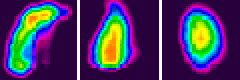
\includegraphics[width=6.00in]
{spiricon/spiricon.png}\\
\caption[Transverse beam profiles from Spiricon camera]{Transverse beam profiles from Spiricon camera. The center image was taken at the apparent waist (downstream from the 2 m lens), the left image was taken 12 inches downstream from the apparent waist, the right image was taken 12 inches upstream from the apparent waist.}
\label{spiricon}
\end{figure} 
%----------------------------------------------------------------------------

%----------------------------------------------------------------------------
As a check, we obtain a similar set of beam profiles using a superposition of the first 4 modes in the Hermite-Gauss expansion. The complex amplitude for the Hermite-Gauss beam is \cite{Siegman:1986a}
%----------------------------------------------------------------------------
%----------------------------------------------------------------------------
%----------------------------------------------------------------------------
\begin{equation}
U_{\ell,m}(x,y,z)
=
A_{\ell,m}
\cdot
\frac{\sqrt{2}}{2^{m+\ell}m!\ell!}
\cdot
\frac
{w_0}
{w(z)}
\cdot
G_{\ell}
\left(
\frac
{\sqrt{2}x}
{w(z)}
\right)
\cdot
G_{m}
\left(
\frac
{\sqrt{2}y}
{w(z)}
\right)
\cdot
\Phi(x,y,z)
\end{equation}
%----------------------------------------------------------------------------
where
%----------------------------------------------------------------------------
\begin{equation}
\Phi(x,y,z)
=
\exp{
\left(
-ikz
-
ik\frac{x^2+y^2}{2R(z)}
+
i(\ell+m+1)
\zeta(z)
\right)
},
\end{equation}
%----------------------------------------------------------------------------
\begin{equation}
G_n(u)
=
H_n(u)
\exp
\left(
\frac
{-u^2}
{2}
\right),
\quad
n=0,1,2\ldots,
\end{equation}
%----------------------------------------------------------------------------
\begin{equation}
\zeta(z)
=
\arctan
\left(
\frac{z}{z_0}
\right),
\end{equation}
%----------------------------------------------------------------------------
$H_n(u)$ is the nth Hermite polynomial, and $A_{\ell,m}$ are the complex expansion coefficients.

It was found with some trial and error that the following set of expansion coefficients generated a composite beam which has a similar profile to the raw dye laser beam as seen on the Spiricon camera:
%----------------------------------------------------------------------------
\begin{eqnarray}
A_{0,0} &=& 5\exp{(-i0.02\pi)}\\
A_{0,1} &=& 1.4\exp{(i0.4\pi)}\\
A_{1,0} &=& 1.8\exp{(i1.6\pi)}\\
A_{1,1} &=& 1.5\exp{(i0.5\pi)},
\end{eqnarray}
%----------------------------------------------------------------------------
see figure \ref{hermite-gauss}. Thus, even though these results are consistent with $M^2\sim1$--$2$, we see that odd shaped non--uniform anti-symmetric beam profiles can result.
%----------------------------------------------------------------------------
% hermite-gauss.tex
% by Troy Hix, May 2005
%----------------------------------------------------------------------------
\begin{figure}
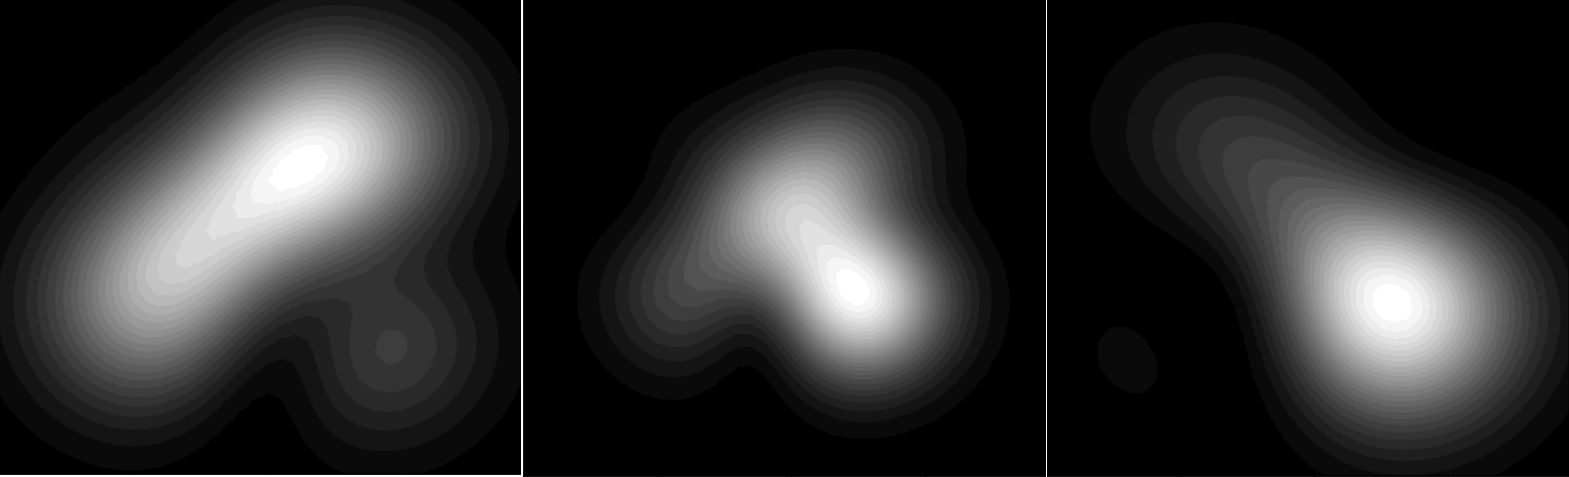
\includegraphics[width=6.00in]
{hermite-gauss/hermite-gauss.png}\\
\caption[Superposition of the first four Hermite-Guass modes]{Superposition of the first four Hermite-Guass modes. the left image is 0.3 m downstream from the waist, the center image is at the waist, the right image is 0.3 m upstream from the waist.}
\label{hermite-gauss}
\end{figure} 
%----------------------------------------------------------------------------


%----------------------------------------------------------------------------
%----------------------------------------------------------------------------
%----------------------------------------------------------------------------
%----------------------------------------------------------------------------
%----------------------------------------------------------------------------

%----------------------------------------------------------------------------
%----------------------------------------------------------------------------
\section{Dye laser output axial mode structure}
The effects of the multi--mode nature of the dye laser output is observed and the RF intensity fluctuations recorded in the output of a square law detector. A RF receiver is used to spectrally analyze the detector output; and it is seen that many discrete spectral features exist out to the high frequency limit of the receiver. This measurement implies the dye laser runs multi--mode with as many as eight characteristic frequencies. Broad multi--mode laser output is not conducive to transition selection in the relatively dense energy structures of molecules.
%----------------------------------------------------------------------------
\subsection{Mode beating}
%----------------------------------------------------------------------------
%----------------------------------------------------------------------------
The YAG--pumped dye laser system produces 8 ns pulses at 20 Hz - in the transform limit, these pulses should have a spectral width of 55 MHz. In fact, the manufacturer of the dye lasers claims the spectral width of each laser pulse to be 1 GHz with axial modes separated by 600 MHz. These specifications are assumed to not be base on measurement (they could not produce hard data), so we assume they arrived at these numbers through some calculation. For example, with a quick glance at the dye laser cavity, one can see that its approximate length is 30 cm. This corresponds to an axial mode spacing of 500 MHz which is consistent with the manufacture's claim.

If the dye laser output contains multiple longitudinal modes, this should show up as ``beating'' in the intensity profile. This can be seen by direct observation of the laser output on a square law detector using an oscilloscope; however, this method is usually limited by the bandwidth of the scope. For example, if the manufacture's claim is true and the dye laser output has 2 or 3 axial modes separated by 600 MHz, then we should see intensity beats at 600 MHz and 1200 MHz - this is beyond the bandwidth of typical oscilloscopes. However, when analyzed with a narrow band RF receiver, there should be 1 or 2 spectral features (in addition to the ``DC'' feature) at 600 MHz and 1200 MHz - well within the bandwidth of the RF receivers we have in the lab. See the discussion in Chapter 19 in reference \cite{Siegman:1986a}.
%----------------------------------------------------------------------------
%----------------------------------------------------------------------------

%----------------------------------------------------------------------------
\subsection{Apparatus}
%----------------------------------------------------------------------------
%----------------------------------------------------------------------------
%----------------------------------------------------------------------------
The dye lasers used here are the Sirah Laser model PRSC-D-24 (dye \#22 and dye \#23) with the Lambda Lock feature. In addition to electrical power and computer control, these dye lasers require an external ``pump'' laser beam to run. The pump laser is the Continuum Powerlite Precision II Scientific Laser System: a Q-switched Nd:YAG laser running at the second harmonic (532 nm). The output of the YAG is split three ways and transported to the inputs of three dye lasers - the beam is stopped before the laser (dye \#21) not being used. DCM dye, from Exciton, was dissolved in Methanol to produce the 628 nm beam used in this experiment. The resulting dye laser output has the following properties: linearly polarized (vertical), 20 Hz repetition rate, $\sim$8 ns FWHM, and a pulse energy of about 58 mJ (38 mJ) for dye \#22 (dye \#23) at the laser output port.

%----------------------------------------------------------------------------
%----------------------------------------------------------------------------

%----------------------------------------------------------------------------
%----------------------------------------------------------------------------
The detector used here is the Hamamatsu R1193U-03 photodiode (S/N 903). The key characteristic is that it has a large active surface area: about 2 cm in diameter. Thus, since our beam is less than 0.5 cm in diameter, we can be sure that a majority of the beam is incident on the active portion of the photodiode to eliminate transverse mode beating \cite{Siegman:1986a}. Since only low light levels should be used with this photodiode, the signal from the photodiode was kept below 1 V (into 50 $\Omega$) even for low duty cycle laser output from the dye lasers. In this way we ensure there will be no damage to the large active area of the photodiode and its sensitivity will remain uniform over the entire area.

%----------------------------------------------------------------------------
%----------------------------------------------------------------------------
%----------------------------------------------------------------------------

%----------------------------------------------------------------------------
%----------------------------------------------------------------------------
The Tektronix 7L14 and the 7L12 Spectrum Analyzers are both used here to process the signal from the photodiode. The key characteristics are their operating ranges: 1 kHz to 2.5 GHz for the 7L14 and 0.1 MHz to 1.8 GHz for the 7L12. For these data the largest resolution bandwidth, 3 MHz, is used. The output is designed to preserve Parseval's Theorem for RF electronic signals: mathematically, the output is the input's Fourier transform squared; i.e. the RF receiver's output voltage is proportional to the \emph{square} of the input voltage. Thus, since the current from the photodiode is proportional to the incident intensity of the optical signal, the receiver's output is proportional to the \emph{square} of the optical intensity. If a beam with a Gaussian intensity profile FWHM of $\sigma_t$ is incident the photodiode, it can be shown that 
%----------------------------------------------------------------------------
\begin{equation}
\delta_{\nu}
=
\frac
{\ln(16)}
{\sqrt{2}\pi\sigma_t}
\label{receiver width}
\end{equation}
%----------------------------------------------------------------------------
where $\delta_{\nu}$ is the FWHM of the resulting spectral profile generated by the RF receiver. Compare this relationship to Equation \ref{FWHM power}.

To calibrate the scans, an accurate reading of the RF receiver center frequency must be acquired. The local oscillator output from the receiver is connected to a Tektronix TR 501 tracking generator. The generator produces a signal with a frequency identical to that of the receiver local oscillator. This signal is analyzed by a Hewlett Packard 53132A universal counter, thus the center frequency of the RF receiver can be directly observed on the counter readout. The tracking generator has a smaller operating range than the 7L14 receiver, however, and can only report accurately on frequencies less than 1.8 GHz. The calibration was linearly extrapolated for frequencies above 1.8 GHz for data taken with the 7L14.

%----------------------------------------------------------------------------
%----------------------------------------------------------------------------
%----------------------------------------------------------------------------
%----------------------------------------------------------------------------
%----------------------------------------------------------------------------

%----------------------------------------------------------------------------
%----------------------------------------------------------------------------
\begin{figure}
\begin{center}
\leavevmode
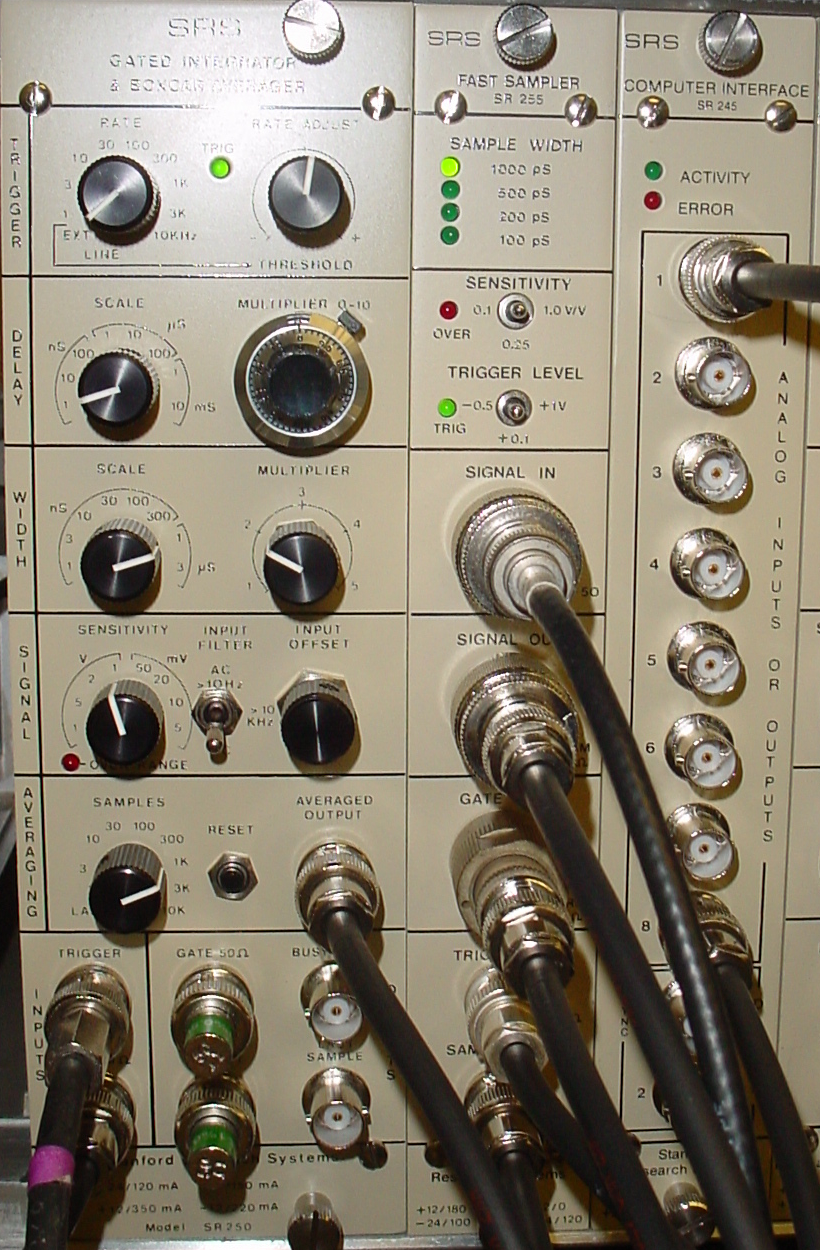
\includegraphics[width=4in]
{boxcar/boxcar.png}\\
\end{center}
\caption[Stanford Research Systems Modules]{Stanford Research Systems Modules. On the left is the SR250: sensitivity = 0.1 V, samples = 1K. In the middle is the SR255: sensitivity = 0.25 V, gate width = 1000 ns. On the right is the SR245: channel one = signal, channel eight = voltage ramp out.}
\label{boxcar}
\end{figure} 
%----------------------------------------------------------------------------

%----------------------------------------------------------------------------
\subsection{Photodiode calibration}
%----------------------------------------------------------------------------
%----------------------------------------------------------------------------
%bb defines the bounding box for the pdf
%viewport defines the area of the pdf used
%in sidewaysfigure the last entry in bb moves the caption toward/away the pic
%in sidewaysfigure the second entry in bb moves the pic toward/away the caption
%----------------------------------------------------------------------------
\begin{figure}
\scalebox{0.6}[0.6]{
\includegraphics*[bb=12 67 665 429]
{PD_cal_block/PD_cal_block.pdf}
}
\caption[Photodiode calibration block diagram]{Photodiode calibration block diagram.}
\label{PD_cal_block}
\end{figure}
%----------------------------------------------------------------------------

%----------------------------------------------------------------------------
This calibration procedure was motivated by a need to measure the radio frequency (RF) power spectrum distribution of the intensity profile of a pulsed dye laser's output. When analyzing these data it is desirable to have the spectral response curve for the photodiode used to observe this intensity profile. Given this curve, we could compare power amplitudes observed within spectral windows at various (differing) regions in the operating range of the photodiode. By exposing the photodiode to light with a white RF spectrum, we can directly measure this response curve using an RF receiver. Better yet, we may assume an equivalent circuit for the photodiode and fit the transfer function of this circuit to the RF receiver data; and thus obtain an analytic form for the response curve. This analytic from can be used to scale the raw data from the RF receiver/photodiode when measuring the RF spectrum of the dye laser output.

Suppose light from a hot filament is incident on a square law detector. If we assume the incident light originates at a black body source, it follows that the spectral power distribution is relatively flat in the radio frequency (RF) region - say from 100 MHz to 2 GHz. Thus, measuring the power within some small bandwidth across this RF region will reveal the transfer function of the photodiode and coupling circuit.

%----------------------------------------------------------------------------
%----------------------------------------------------------------------------
%bb defines the bounding box for the pdf
%viewport defines the area of the pdf used
%in sidewaysfigure the last entry in bb moves the caption toward/away the pic
%in sidewaysfigure the second entry in bb moves the pic toward/away the caption
%----------------------------------------------------------------------------
\begin{figure}
\scalebox{0.75}[0.75]{
\includegraphics*[bb=94 217 611 521]
{PD_fit/PD_fit.pdf}
}
\caption[Photodiode calibration fit]{Photodiode calibration fit. The fit may be used to scale the output from the RF receiver/photodiode output to give realistic relative amplitudes over the operating range of the instrument}
\label{PD_fit}
\end{figure}
%----------------------------------------------------------------------------

%----------------------------------------------------------------------------
The light source in this experiment is a automotive style filament light bulb. The bulb was mounted in a desktop style lamp and plugged into a regular AC outlet. The switch on the lamp had three settings: ``off'' ``low'' and ``high''; the ``high'' setting is used here. The bulb's output is filtered through a yellow gelatin filter sheet (before being focused by a +30 mm lens) to limit the energy spread of the electrons emitted from the photocathode: this will optimize the photodiode bandwidth by reducing transit time effect to a minimum. See Figure \ref{PD_cal_block} for a block diagram of the calibration procedure.

The Hamamatsu R1193U-03 photodiode (S/N 878) is used here. Its key characteristics are its large active surface area (about 2 cm in diameter) and its fast response time. Some specifications from a reseller's site (Sphere Research Corporation) are: ``High performance, bi-planar, ultra-fast phototube (270ps risetime, 100ps fall time) with integral light shield and lab housing (with tripod mount and connectors). UV sensitive, linearized for laser power detection, details coming from Hamamatsu, 2.5KV typical excitation.''

The voltage-gain transfer function for the equivalent circuit of the photodiode and associated coupling circuit is (personal communication, John M. J. Madey, July 2005)
%----------------------------------------------------------------------------
\begin{equation}
\frac{
V_{out}}{
V_{in}
}
=
\frac
{1}
{1 + i \omega C ( 25 + i \omega L )}
\label{transfer function}
\end{equation}
%----------------------------------------------------------------------------
where $V_{out}$ is the voltage seen across the 50 $\Omega$ external load resistor, ${V_{in}}$ is the voltage across the capacitor (photodiode gap), C is the capacitance of this ``gap'', and L is the inductance associated to the photodiode. See Figure \ref{PD_fit} for a plot of the data and the fit.

%----------------------------------------------------------------------------
%----------------------------------------------------------------------------

%----------------------------------------------------------------------------
\subsection{Experiment layout}
%------------------------------------------------------------------------------
%------------------------------------------------------------------------------
The beam line used here is similar to the one described in Section \ref{sample layout} except the attenuators are not used and in its place we use a pair of crossed polarizers (polarizing cube beam splitters) and a Pockels cell. The system has an extinction ratio of about 200:1 (see UH notebook UH-018 page 65) and produces a pulse with a FWHM of about 4 ns. Before the Pockels cell we have about 5.4 mJ, thus after the Pockels cell (heading toward the +750 mm lens) is about 27 uJ. The dye laser is tuned to 535.893 nm (a targeted absorption line) and the monochromator is tuned to capture a single LIF line at 632.9 nm. Again the signal from the PMT at the output of the monochromator is scanned (temporal gate scan) and averaged with a boxcar averager.

The measurement has facilitated the development of the data acquisition system required for lifetime measurements. The boxcar averager works at the 1000 ps gate width setting (it has settings down to 100 ps, but these have not been tried) and the LabView program records the data as a convenient text file. We have also discovered that the intensity fluctuations of the dye laser output introduce unwanted jitter in the position of the trigger relative to the peak -- accurate lifetime measurements will require a way to eliminate the jitter or, better yet, reduce the intensity fluctuations in the input beam. Contamination of the cell may have introduced additional channels through which the iodine can decay. A clean loading method must be developed in order to isolate and measure specific effects on the fluorescence decay.
%------------------------------------------------------------------------------
%------------------------------------------------------------------------------
%------------------------------------------------------------------------------
%------------------------------------------------------------------------------
%------------------------------------------------------------------------------
%------------------------------------------------------------------------------

%----------------------------------------------------------------------------
\subsection{Data acquisition}
%----------------------------------------------------------------------------
%----------------------------------------------------------------------------
%----------------------------------------------------------------------------
Four data sets (1 hour each) are taken with the 7L12 receiver. First, dye laser \#22 is scanned; next the beam is blocked for another 1 hour scan; then dye laser \#23 is scanned; finally the YAG seeder is turned off and dye \#23 is scanned again. Before each dye laser scan, the polarizers are adjusted so that the signal from the photodiode has an approximate amplitude of 100 mV. The 7L12 settings are as follows: amplifier set to its 5th notch, attenuator at 0 dB (together the amplifier and attenuator give a reference level of -70 dB), the video filter is active, FREQ SPAN/DIV is MAX (1.8 GHz), bandwidth 3 MHz, scale is linear (not log). The SR250 settings are as follows: gate width 300 ns, sensitivity 5 mV, samples 100. The computer settings are as follows: number of points acquired is set to 4000, the scan length is 3600 seconds, and the voltage ramp range is 0.5 - 10 volts.

Three data sets (1 hour each) are taken with the 7L14 receiver. First, dye laser \#23 is scanned; next the beam is blocked for another 1 hour scan; finally dye laser \#22 is scanned. Before each dye laser scan, the polarizers are adjusted so that the signal from the photodiode has an approximate amplitude of 15 mV (the 7L14 is more sensitive than the 7L12). The 7L14 settings are as follows: amplifier set to its 5th notch, attenuator at 0 dB (together the amplifier and attenuator give a reference level of -70 dB), the video filter is active, FREQ SPAN/DIV is MAX (2.5 GHz), bandwidth 3 MHz, scale is linear (not log). The SR250 settings were not changed. On the computer the voltage ramp was changed to 0.9 - 10 volts.

%----------------------------------------------------------------------------
%----------------------------------------------------------------------------

%----------------------------------------------------------------------------
\subsection{Data analysis}
%----------------------------------------------------------------------------
%----------------------------------------------------------------------------
First, the raw data sets are calibrated. The computer records the voltage sampled from the SR250 verses the associated voltage level sent to the receiver from the voltage ramp. The relationship between voltage sent to the receiver and the corresponding center frequency of the receiver is obtained by taking pictures of the laptop computer next to the HP 53132A counter. Each picture shows the current voltage on the voltage ramp (displayed on the laptop screen) and the current center frequency of the receiver. Several such pictures are taken during each scan. The relationship is found to be very linear, but shifts a little bit from scan to scan.

Once calibrated, each scan is scaled to compensate for the response curve of the photodiode (see AHI02-DN3300-5-VR08). Only one of the two photodiodes was calibrated (S/N 878) - here we use the one that wasn't calibrated and assume it has a similar response. See Figs. \ref{22-12}
%----------------------------------------------------------------------------
%----------------------------------------------------------------------------
%bb defines the bounding box for the pdf
%viewport defines the area of the pdf used
%in sidewaysfigure the last entry in bb moves the caption toward/away the pic
%in sidewaysfigure the second entry in bb moves the pic toward/away the caption
%----------------------------------------------------------------------------
\begin{figure}
\scalebox{0.8}[0.6]{
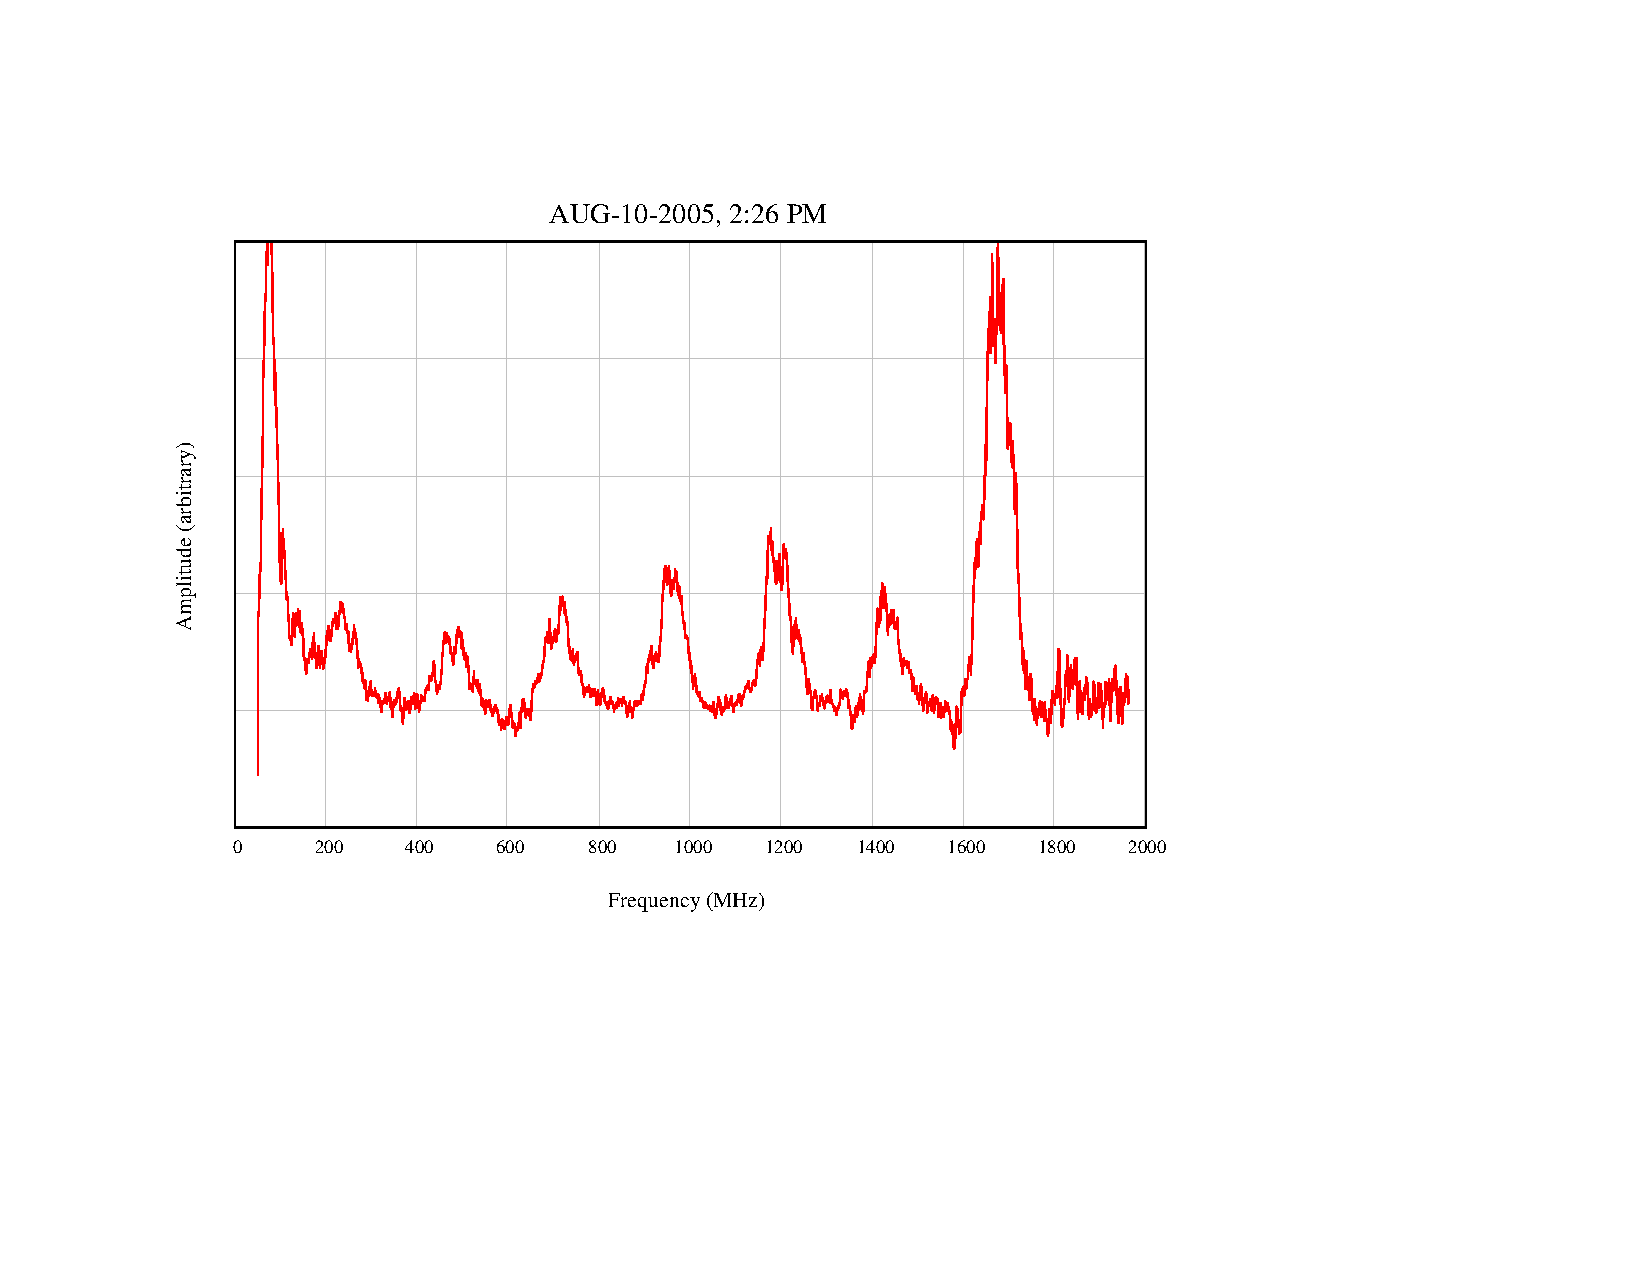
\includegraphics[viewport=150 200 300 450, bb=85 160 300 550]
{22-12/22-12.pdf}
}
\caption{Dye laser \#22 scanned with the 7L12}
\label{22-12}
\end{figure}
%----------------------------------------------------------------------------

%----------------------------------------------------------------------------
and \ref{22-14}
%----------------------------------------------------------------------------
%----------------------------------------------------------------------------
%bb defines the bounding box for the pdf
%viewport defines the area of the pdf used
%in sidewaysfigure the last entry in bb moves the caption toward/away the pic
%in sidewaysfigure the second entry in bb moves the pic toward/away the caption
%----------------------------------------------------------------------------
\begin{figure}
\scalebox{0.8}[0.6]{
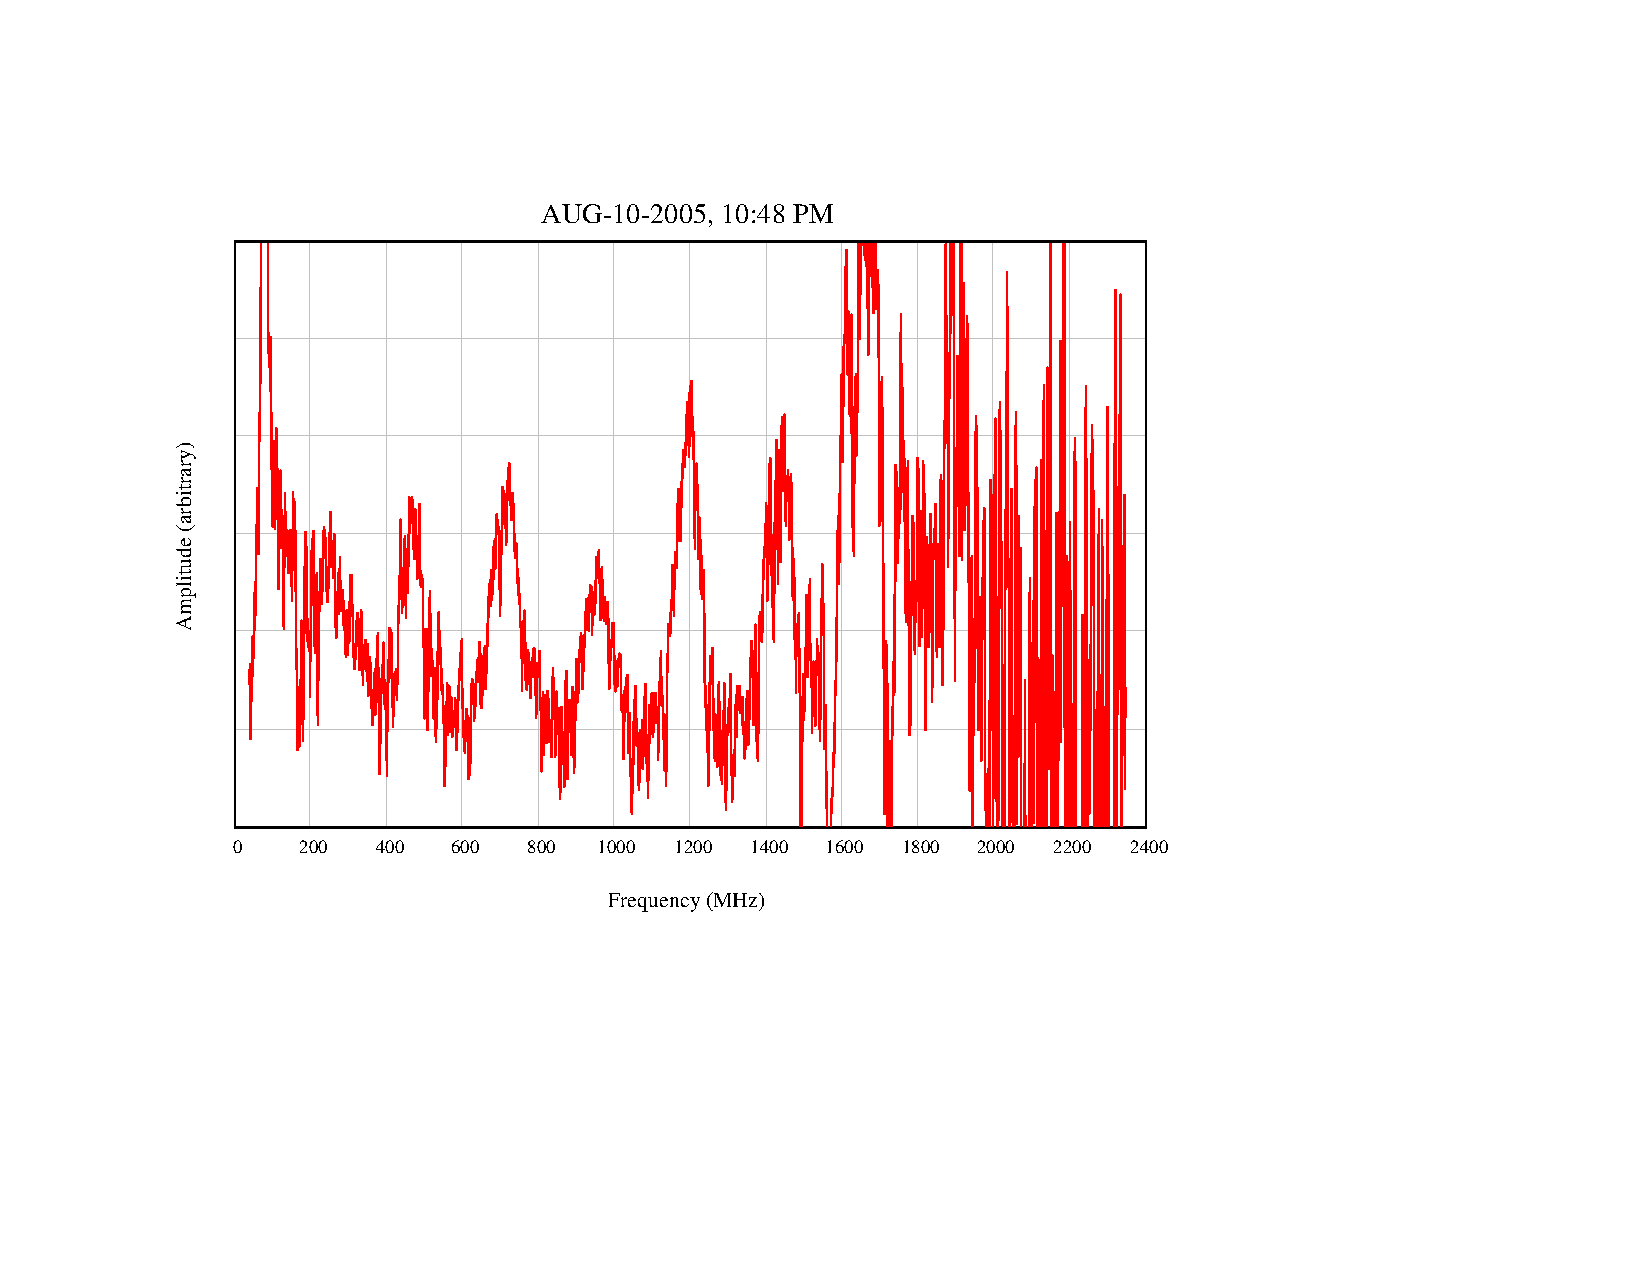
\includegraphics[viewport=150 200 300 450, bb=85 160 300 550]
{22-14/22-14.pdf}
}
\caption{Dye laser \#22 scanned with the 7L14}
\label{22-14}
\end{figure}
%----------------------------------------------------------------------------

%----------------------------------------------------------------------------
to see the data for dye laser \#22 taken with the 7L12 and 7L14 respectively. See Figs. \ref{23-12}
%----------------------------------------------------------------------------
%----------------------------------------------------------------------------
%bb defines the bounding box for the pdf
%viewport defines the area of the pdf used
%in sidewaysfigure the last entry in bb moves the caption toward/away the pic
%in sidewaysfigure the second entry in bb moves the pic toward/away the caption
%----------------------------------------------------------------------------
\begin{figure}
\scalebox{0.8}[0.6]{
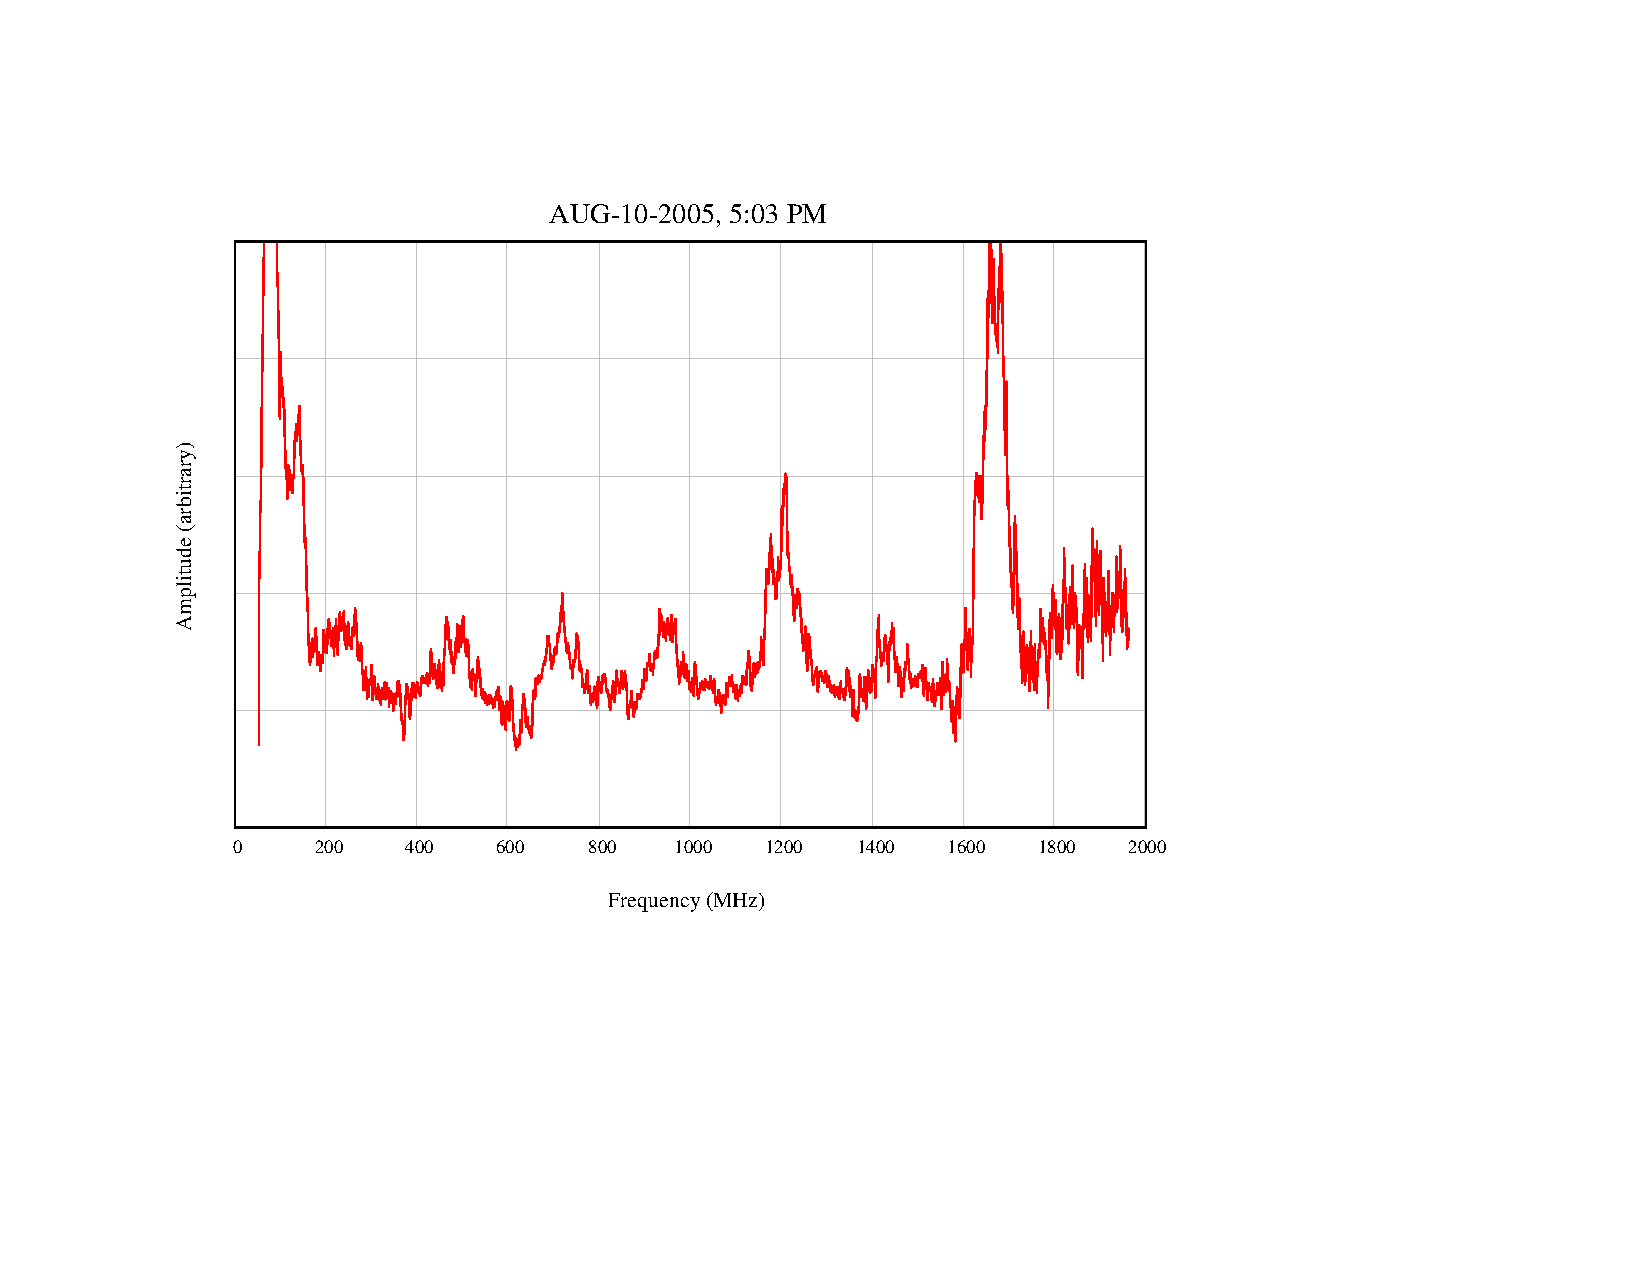
\includegraphics[viewport=150 200 300 450, bb=85 160 300 550]
{23-12/23-12.pdf}
}
\caption{Dye laser \#23 scanned with the 7L12}
\label{23-12}
\end{figure}
%----------------------------------------------------------------------------

%----------------------------------------------------------------------------
and \ref{23-14}
%----------------------------------------------------------------------------
%----------------------------------------------------------------------------
%bb defines the bounding box for the pdf
%viewport defines the area of the pdf used
%in sidewaysfigure the last entry in bb moves the caption toward/away the pic
%in sidewaysfigure the second entry in bb moves the pic toward/away the caption
%----------------------------------------------------------------------------
\begin{figure}
\scalebox{0.8}[0.6]{
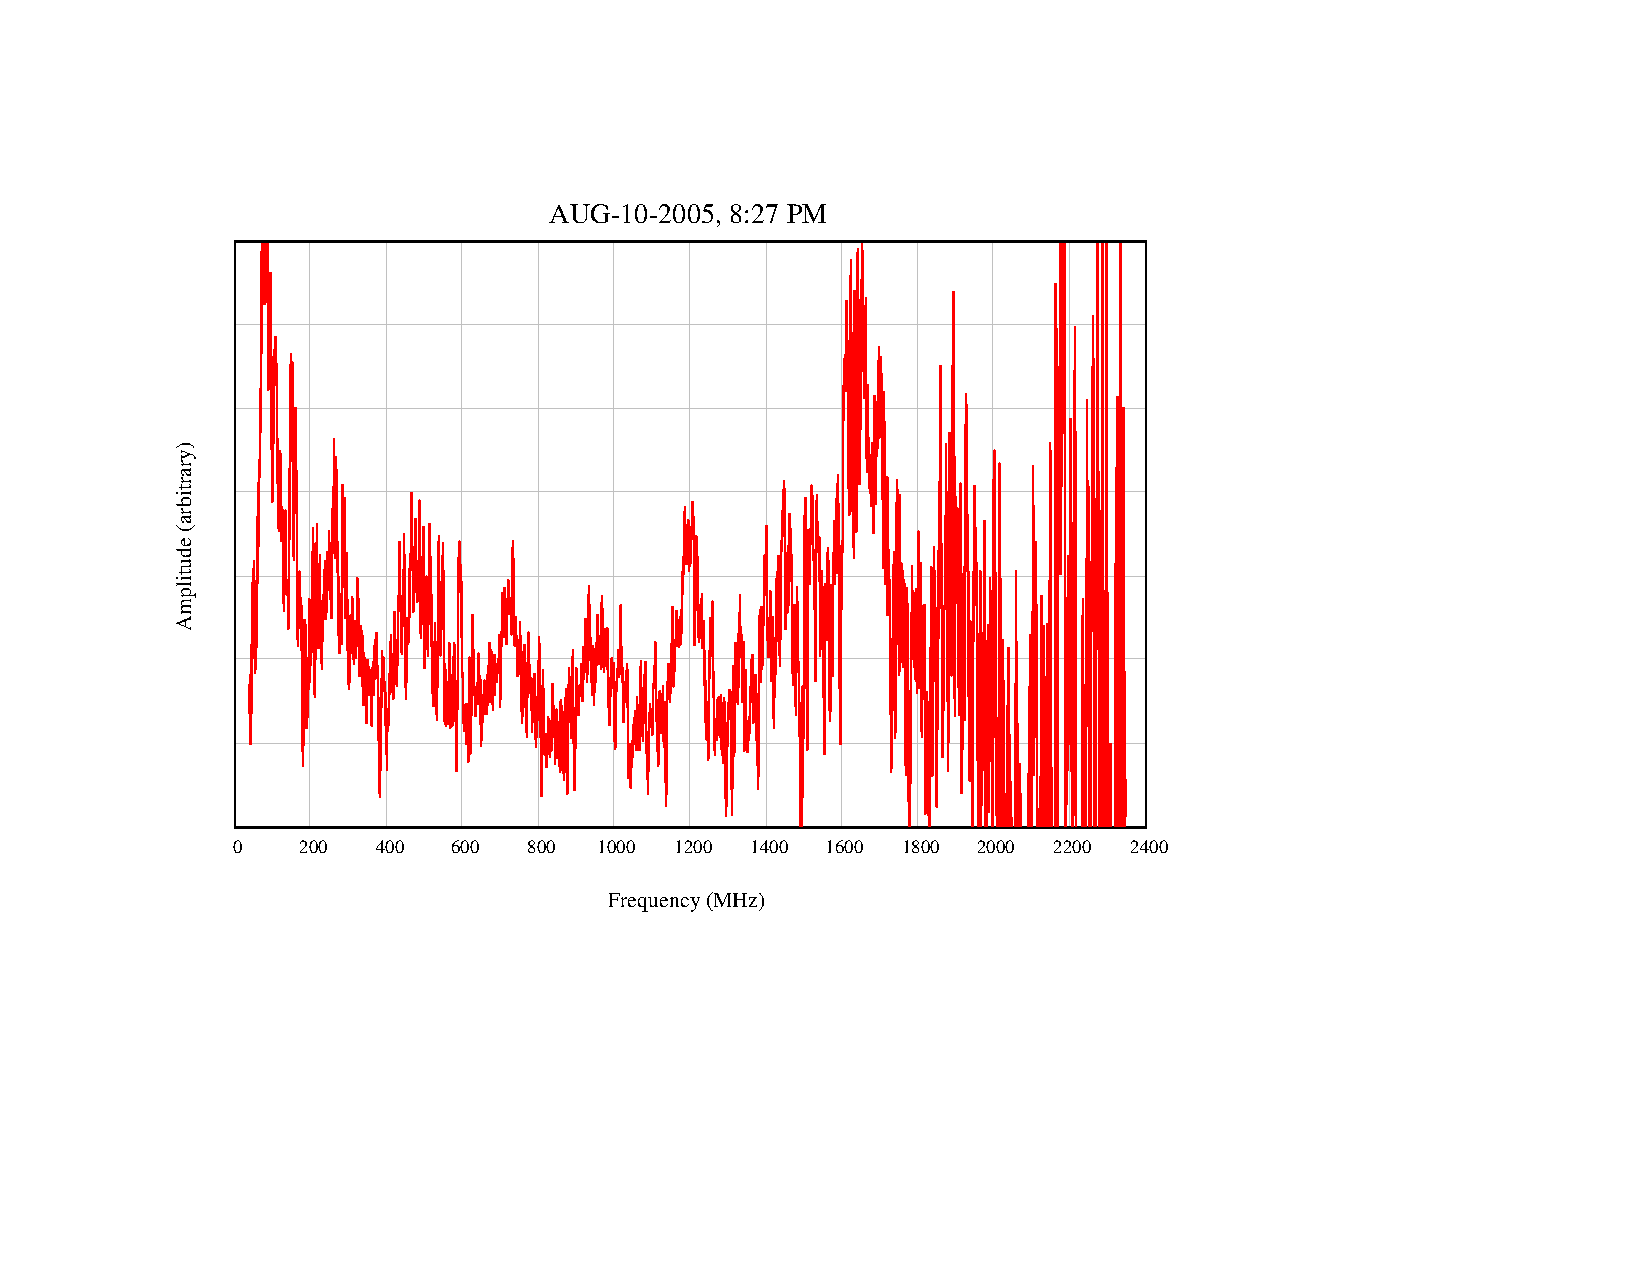
\includegraphics[viewport=150 200 300 450, bb=85 160 300 550]
{23-14/23-14.pdf}
}
\caption{Dye laser \#23 scanned with the 7L14}
\label{23-14}
\end{figure}
%----------------------------------------------------------------------------

%----------------------------------------------------------------------------
to see the data for dye laser \#23 taken with the 7L12 and 7L14 respectively. The following overlays are of the raw data - calibrated but not scaled for the photodiode response. Figs. \ref{2X-12}
%----------------------------------------------------------------------------
%----------------------------------------------------------------------------
%bb defines the bounding box for the pdf
%viewport defines the area of the pdf used
%in sidewaysfigure the last entry in bb moves the caption toward/away the pic
%in sidewaysfigure the second entry in bb moves the pic toward/away the caption
%----------------------------------------------------------------------------
\begin{figure}
\scalebox{0.8}[0.6]{
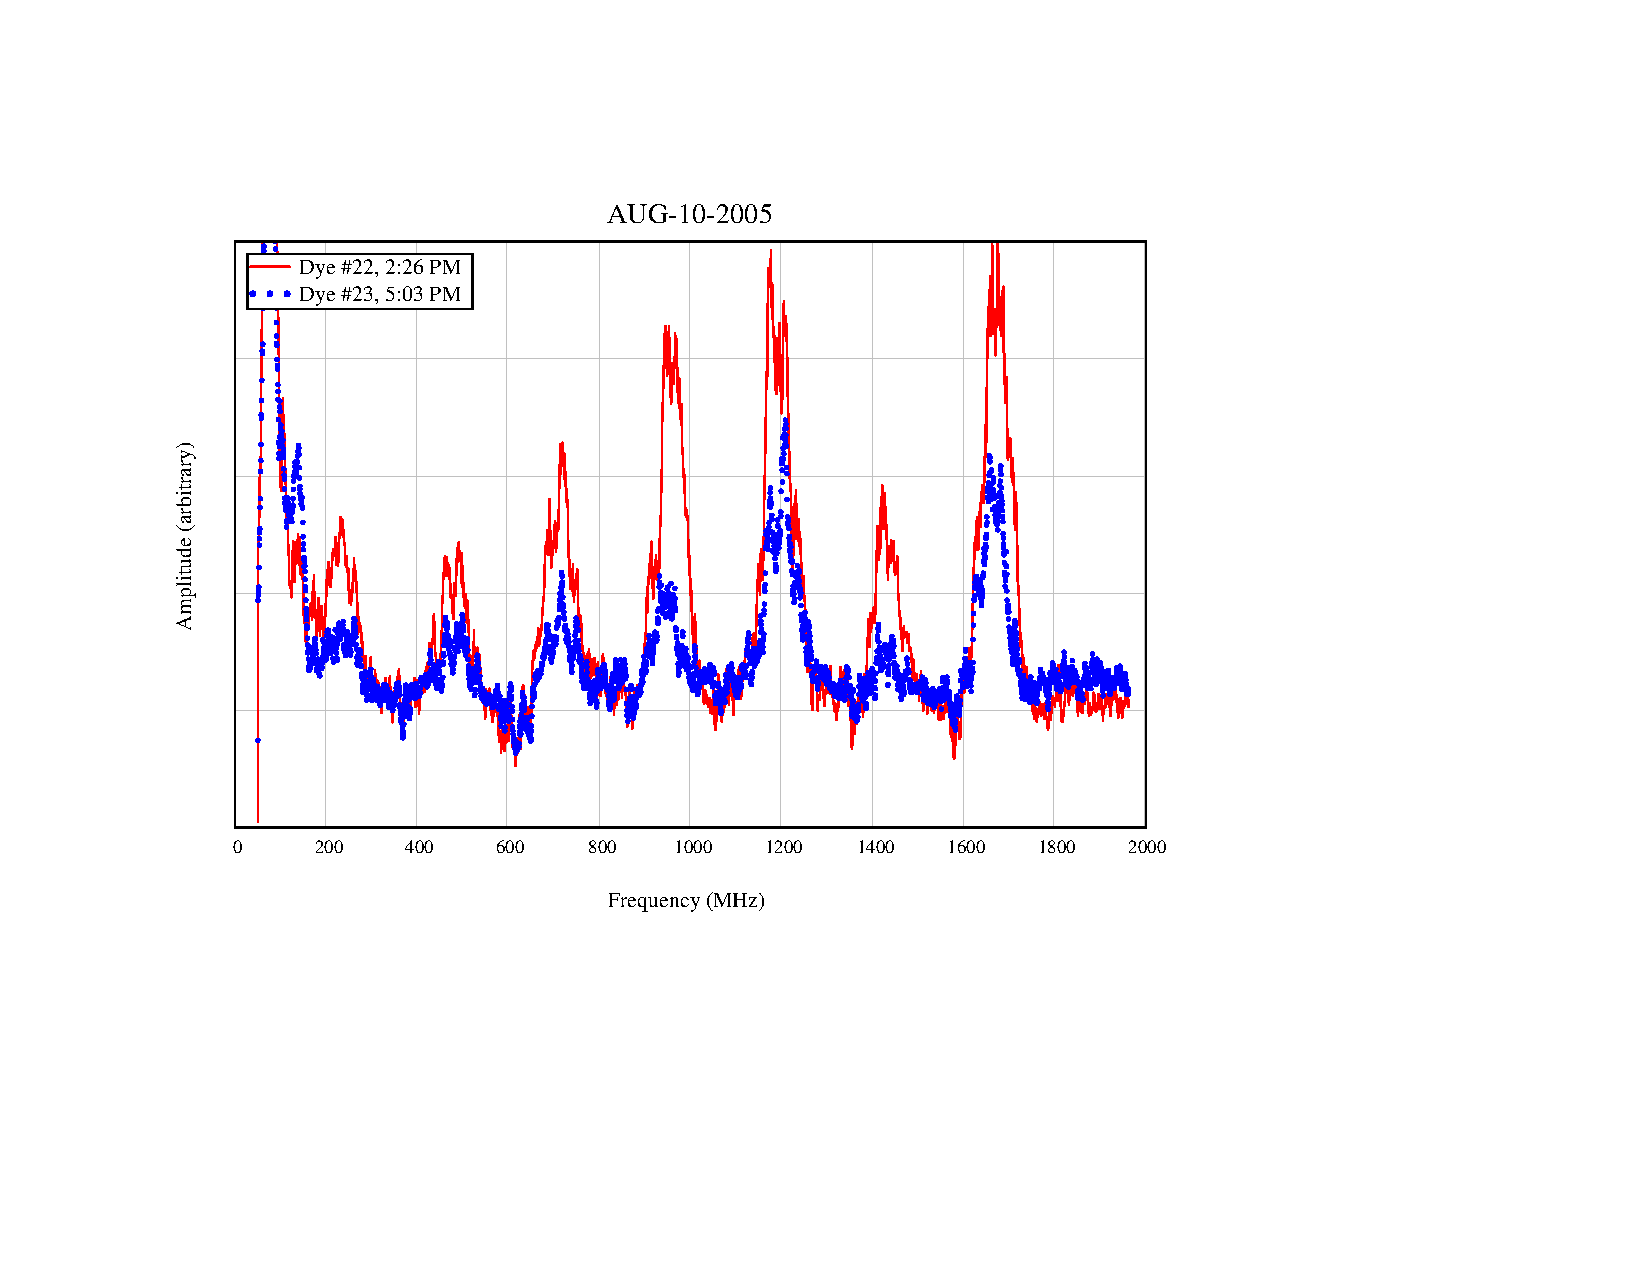
\includegraphics[viewport=150 200 300 450, bb=85 160 300 550]
{2X-12/2X-12.pdf}
}
\caption{Both dye lasers scanned with the 7L12 (raw data)}
\label{2X-12}
\end{figure}
%----------------------------------------------------------------------------

%----------------------------------------------------------------------------
and \ref{2X-14}
%----------------------------------------------------------------------------
%----------------------------------------------------------------------------
%bb defines the bounding box for the pdf
%viewport defines the area of the pdf used
%in sidewaysfigure the last entry in bb moves the caption toward/away the pic
%in sidewaysfigure the second entry in bb moves the pic toward/away the caption
%----------------------------------------------------------------------------
\begin{figure}
\scalebox{0.8}[0.6]{
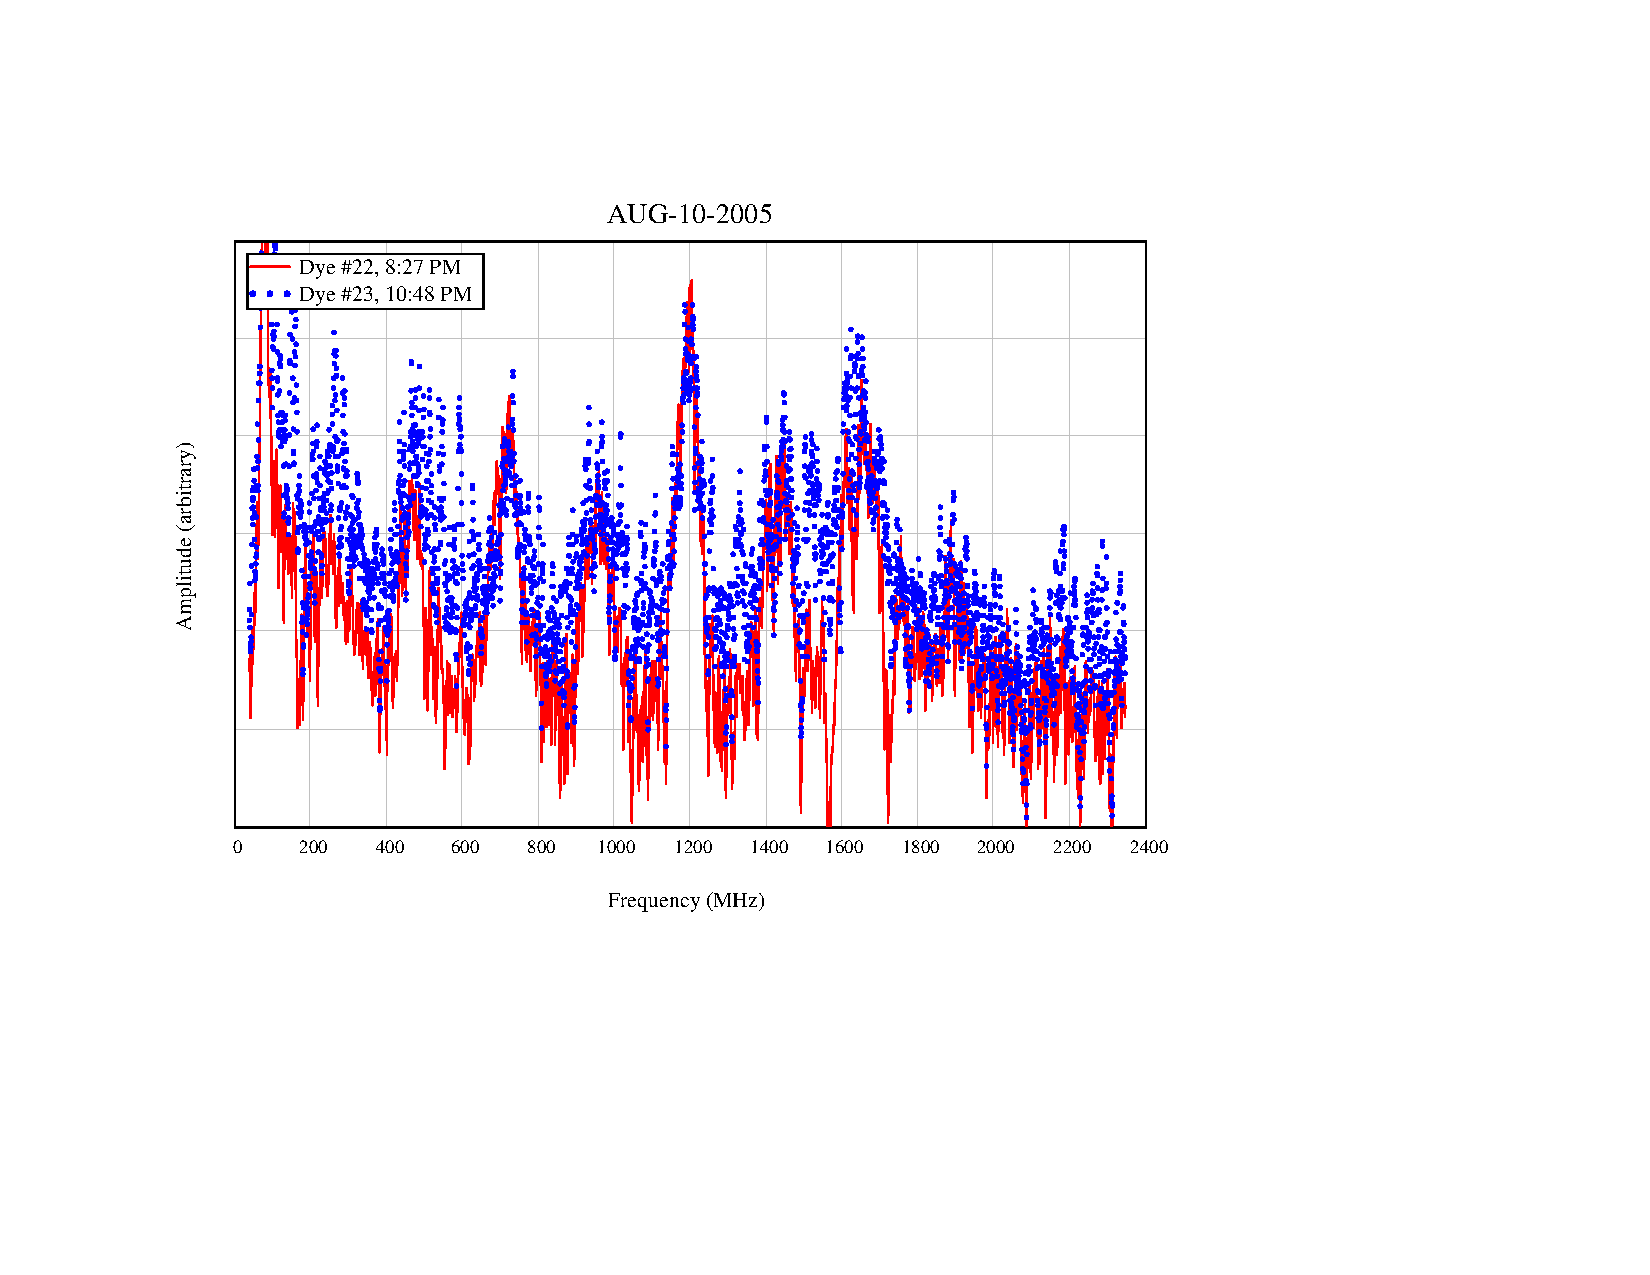
\includegraphics[viewport=150 200 300 450, bb=85 160 300 550]
{2X-14/2X-14.pdf}
}
\caption{Both dye lasers scanned with the 7L14 (raw data)}
\label{2X-14}
\end{figure}
%----------------------------------------------------------------------------

%----------------------------------------------------------------------------
show overlays of the data from the two lasers taken with the 7L12 and 7L14 respectively. Fig. \ref{23-12-seederX}
%----------------------------------------------------------------------------
%----------------------------------------------------------------------------
%bb defines the bounding box for the pdf
%viewport defines the area of the pdf used
%in sidewaysfigure the last entry in bb moves the caption toward/away the pic
%in sidewaysfigure the second entry in bb moves the pic toward/away the caption
%----------------------------------------------------------------------------
\begin{figure}
\scalebox{0.8}[0.6]{
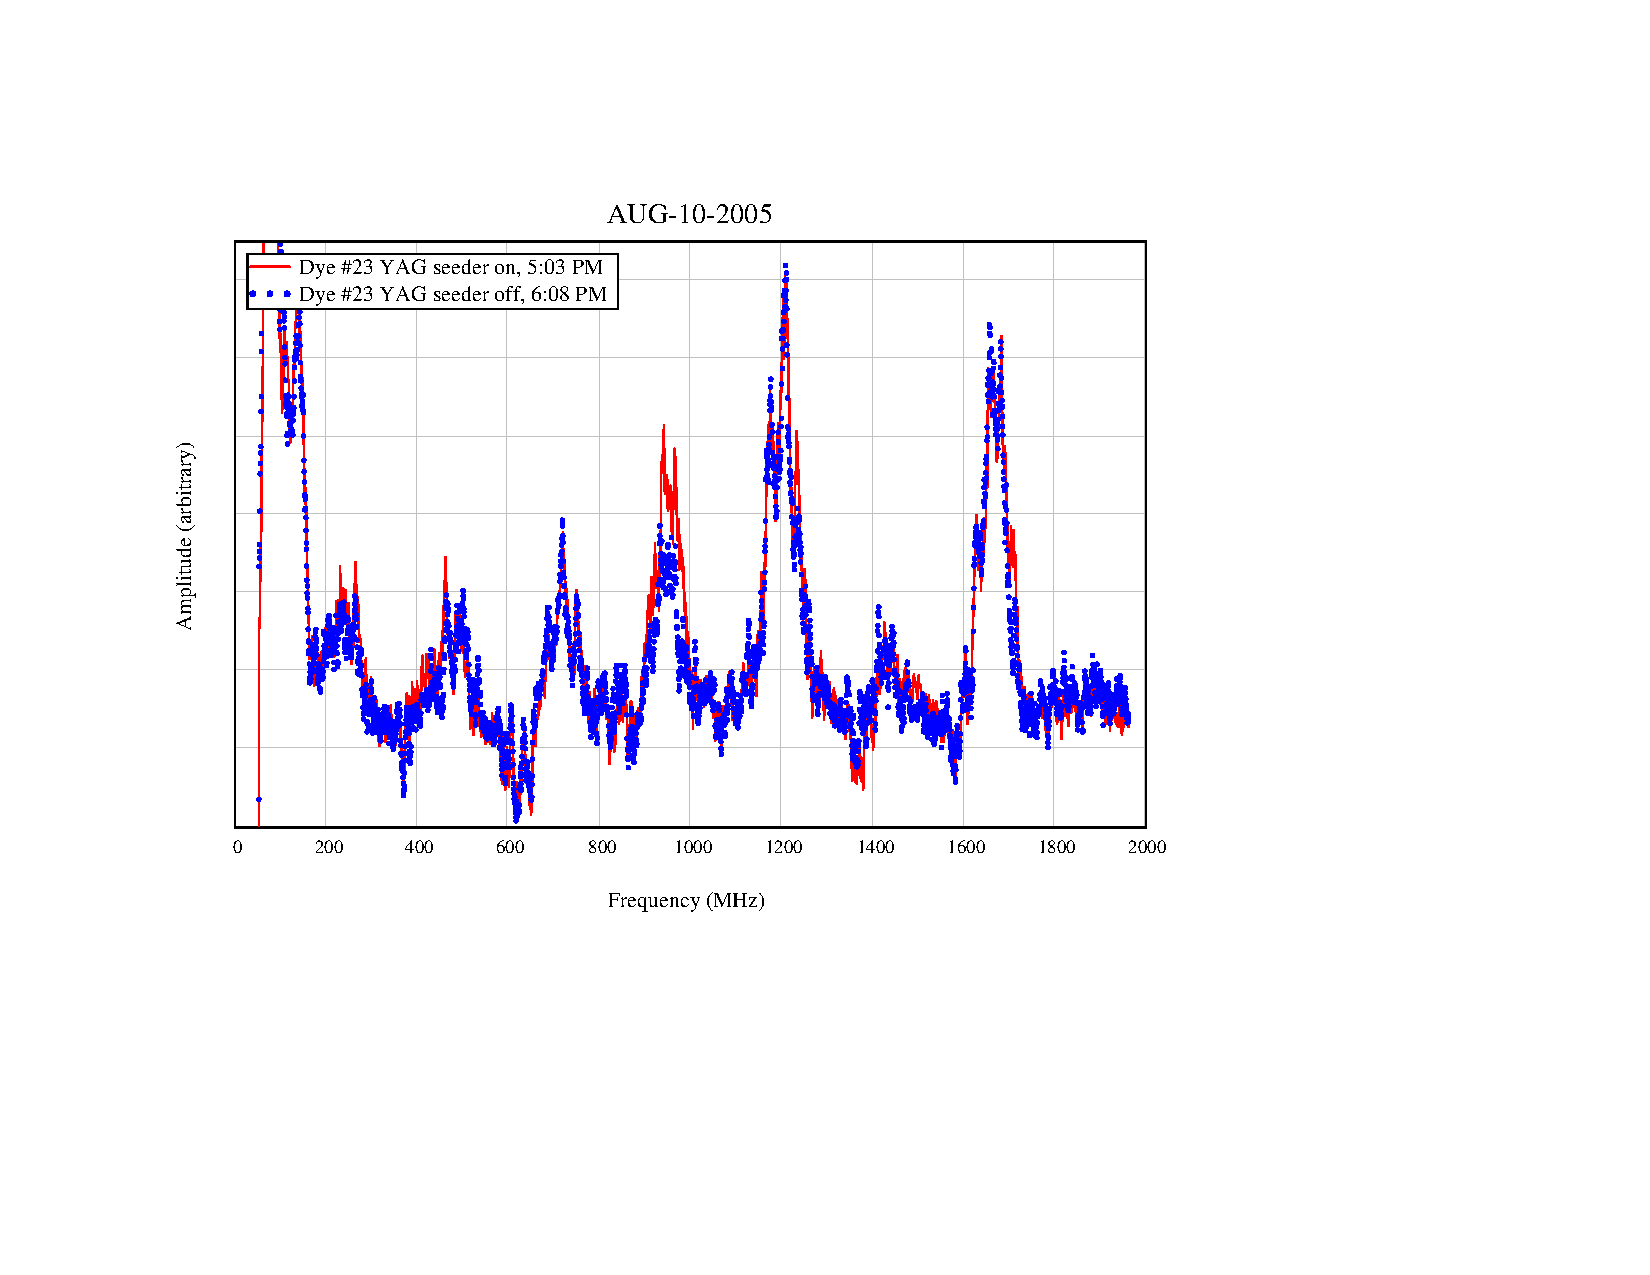
\includegraphics[viewport=150 200 300 450, bb=85 160 300 550]
{23-12-seederX/23-12-seederX.pdf}
}
\caption{Dye laser \# 23, with YAG pump with the seeder on/off, scanned with the 7L12 (raw data)}
\label{23-12-seederX}
\end{figure}
%----------------------------------------------------------------------------

%----------------------------------------------------------------------------
shows an overlay of the data from dye laser \#23 with the YAG pump in two states: seeder on and seeder off.

Finally, to check the spectral width of the observed features, the peak at 1200 MHz from the 7L12 scan of the \#23 dye laser is fit to a Gaussian (see Fig. \ref{fit}).
%----------------------------------------------------------------------------
%----------------------------------------------------------------------------
%bb defines the bounding box for the pdf
%viewport defines the area of the pdf used
%in sidewaysfigure the last entry in bb moves the caption toward/away the pic
%in sidewaysfigure the second entry in bb moves the pic toward/away the caption
%----------------------------------------------------------------------------
\begin{figure}
\scalebox{0.7}[0.7]{
\includegraphics*[bb=75 286 643 540]
{fit/fit.pdf}
}
\caption[Gaussinan fit for a single RF beat spectral feature]{The spectral feature at 1200 MHz fits a Gaussian with a FWHM of 83 MHz. This corresponds to a Gaussian in the time domain with a FWHM of 7.5 ns. This matches the observed pulse width - implying each mode is transform limited.}
\label{fit}
\end{figure}
%----------------------------------------------------------------------------

%----------------------------------------------------------------------------
Using the FWHM from the fit, Eqn. \ref{receiver width} is used to determine the corresponding transform limited temporal width.
%----------------------------------------------------------------------------
%----------------------------------------------------------------------------

%----------------------------------------------------------------------------
%----------------------------------------------------------------------------
\section{Conclusion}
%----------------------------------------------------------------------------
%------------------------------Broad objectives------------------------------
%----------------------------------------------------------------------------
This chapter chronicles the stages of laboratory development undergone over the past few years. The main measurements at each stage were used as a guide to develop the equipment and techniques required for demonstration of molecular control in LIDAR systems.
%----------------------------------------------------------------------------
%----------------------------------So what?----------------------------------
%----------------------------------------------------------------------------

As each stage was completed various components of the apparatus were either designed and assembled or evolved to the next generation. After the installation of the PMT at its output the monochromator served each experiment well until the recent aromatic compound measurements. The Hg pulser and Pockles cell system went through various stages of development starting with the initial tests of the Hg pulser on LED's to the integration of the system with the YAG pumped dye laser system during the fluorescence line decay measurements. The software model was tested at each stage from the familiar non-resonant HeNe LIF to pulsed resonant dye LIF. The data acquisition system was built for the first dye laser experiments and has remained relatively unchanged since then. Recently, a calibration issue with the monochromator self scan feature has prompted the need of a second generation of the data acquisition software.
%----------------------------------------------------------------------------
%---------------------------------Synthesize---------------------------------
%----------------------------------------------------------------------------
%----------------------------------------------------------------------------
%----------------------------------------------------------------------------
%----------------------------------------------------------------------------

%----------------------------------------------------------------------------
%----------------------------------------------------------------------------
%----------------------------------------------------------------------------
